

\section{Поляризационные устройства: кристаллические фазовые пластинки(четверьволновые и полуволновые пластинки), компенсаторы. Призмы Николя, Глана, Волластона. Дихроичные пластинки, поляроиды, принцип действия.}


\subsection{Кристаллические пластинки $\frac{\lambda}{2}$ и $\frac{\lambda}{4}$}

\subsubsection{Определения}

Пусть пластинка вырезана из одноосного кристала параллельно его оси. В такой пластинке обыкновенный и необыкновенный лучи не разделяются, но им отвечаются разные показатели преломления  $n_o$ и $n_e$. Поэтому, пройдя через пластинку, лучи приобретают дополнительную разность хода

\begin{equation*}
    \Delta = h(n_e - n_o)
\end{equation*}

Соответствующая разность фаз равна

\begin{equation*}
    \Delta \phi = \frac{2\pi}{\lambda}h(n_e - n_o)
\end{equation*}

Здесь $\lambda = \frac{2\pi c}{\omega}$ - длина волны света в вакууме.

Рассмотрим два случая.

1. Если

\begin{equation*}
    \Delta = \frac{\lambda}{4} + m\lambda 
\end{equation*}

пластинка называется четвертьволновой. Она вносит дополнительную разность фаз обыкновенного и необыкновенного лучей

\begin{equation*}
    \Delta \phi = \frac{\pi}{2} + 2\pi m  
\end{equation*}

2. Если

\begin{equation*}
    \Delta = \frac{\lambda}{2} + m\lambda 
\end{equation*}

пластинка называется полуволновой. Эта пластинка создает дополнительную разность фаз 

\begin{equation*}
    \Delta \phi = \pi + 2\pi m
\end{equation*}

\subsubsection{Действие четвертьволновой  пластинки}

1. \textit{Волна с круговой поляризацией}

После прохождения такой волной четвертьволновой пластинки она оказывается линейно поляризованной. Действительно, исходная волна описывается формулами

\begin{equation*}
 \begin{cases}
   E_x = E_0 \cos \omega t,
   \\
   E_z = E_0 \cos \omega t.
 \end{cases}
\end{equation*}

Если эту волну пропустить через пластинку $\frac{\lambda}{4}$, то независимо от ориентации пластинки одна компонента излучения оказывается обыкновенным лучом, а другая - необыкновенным. Соответственно после прохождения пластинки между компонентами возникает сдвиг фаз $\frac{\pi}{2}$, а сама уже будет описываться формулами

\begin{equation*}
 \begin{cases}
   E_x = E_0 \cos \omega t,
   \\
   E_z = \pm E_0 \sin \omega t.
 \end{cases}
\end{equation*}
2. \textit{Линейно поляризованная волна}

Если исходная волна была линейно поляризованной, то после прохождения пластинки она превращается в волну с эллиптической поляризацией. Пусть ось кристалла - ось $z$, а плоскость поляризации - $xz$. Тогда линейно поляризованная волна, падающая на пластинку, описывается выражениями

\begin{equation*}
 \begin{cases}
   E_x = E_{x0} \cos \omega t,
   \\
   E_z = E_{z0} \cos \omega t.
 \end{cases}
\end{equation*}

Волна, прошедшая пластинку, будет описываться следующими формулами:

\begin{equation*}
 \begin{cases}
   E_x = E_{x0} \cos (\omega t + \delta),
   \\
   E_z = E_{z0} \cos \left(\omega t + \delta - \frac{\pi}{2} \right).
 \end{cases}
\end{equation*}

Таким образом, мы получили эллиптически поляризованную волну. В частном случае, когда $E_{x0} = E_{z0} \equiv E_0$, прошедшая волна приобретает круговую поляризацию. 
\subsubsection{Действие полуволновой пластинки}

Если падающая волна была линейно поляризованной, то в результате прохождения пластинки $\frac{\lambda}{2}$ меняется плоскость поляризации (см. рисунок). Этот результат объясняется тем, что возникает дополнительный сдвиг фаз обыкновенного и необыкновенного лучей в $\pi$. Это можно интерпретировать так, что просто изменяется знак одной из проекций вектора $E$.


\subsection{Призма Николя}

Для изготовления призмы Николя у продолговатого ромбоэдра, полученного скалыванием из куска исландского шпата, сошлифовывают основания так, чтобы новые основания составляли с боковыми ребрами угол $68^o$. Затем кристалл разрезают вдоль плоскости, перпендикулярной к новым основаниям и к главному сечению кристалла. Отполировав плоскости разреза, оба куска склеивают в прежнем положении тонким слоем канадского бальзама.

\begin{figure}[h!]
    \centering
    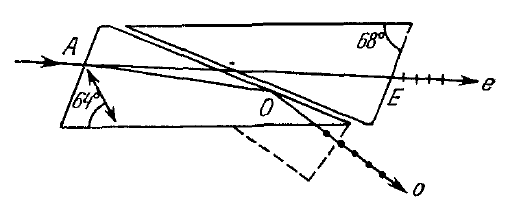
\includegraphics[scale=1]{nicole.png}
    \caption{Призма Николя}
    \label{fig:my_label}
\end{figure} 

На рисунке показано сечение призмы Николя плоскостью главного сечения. Двойная стрелка, наклоненная под углом $64^o$ к длинному ребру, указывает направление оптической оси. Такое обозначение применяется в дальнейшем и для других призм. Луч света, падая на искусственное основание кристалла, разделяется внутри кристалла на обыкновенный $AO$ и необыкновенный $AE$. Показатель преломления канадского бальзама $(n = 1,55)$ имеет промежуточное значение между обыкновенным $(n_o = 1,658)$ и необыкновенным $(n_e = 1,486) $ показателем преломления исландского шпата. Углы в призме Николя рассчитаны так, чтобы необыкновенный луч прошел через слой канадского бальзама, а обыкновенный претерпел на нем полное отражение и поглотился зачерненной боковой гранью. В результате свет, вышедший из призмы, окажется линейно поляризованным.

Призма Николя имеет скошенное основание, что вызывает параллельное боковое смещение падающего луча при прохождении его через призму. Следствием этого является кругообразное перемещение выходящего луча при вращении призмы вокруг ее оси. От этого недостатка избавлена призма Глана, имеющая форму прямоугольного параллелепипеда.

\begin{figure}[h!]
    \centering
    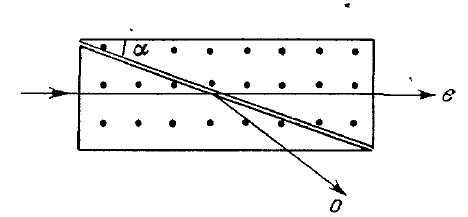
\includegraphics[scale=1]{glan.png}
    \caption{Призма Глана}
    \label{fig:my_label}
\end{figure} 

\newpage

\subsection{Призма Волластона}

Призма Волластона является одной из двулучевых поляризационных призм.  Призма состоит из комбинации стеклянной призмы с кристаллической из исландского шпата, оптическая ось которой параллельна преломляющему ребрую Призмы соприкасаются и склеиваются, как показано на рисунке. Показатель преломления стекла почти точно совпадает с показателем преломления исландского шпата. Падающий пучок неполяризованного света в призме разделяется на обыкновенный и необыкновенный. Выходящие лучи линейно поляризованного света отклоняются в разные стороны.

\begin{figure}[h!]
    \centering
    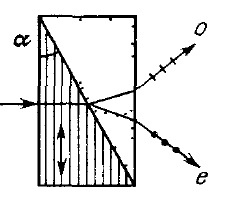
\includegraphics[scale=1]{volastone.png}
    \caption{Призма Волластона}
    \label{fig:my_label}
\end{figure} 

\subsection{Дихроичные пластинки}

У многих кристаллов поглощение света зависит от направления электрического вектора в световой волне. Это являние используется для получения линейно поляризованного света в дихроичных пластинках. К ним относятся, например, пластинки турмалина и поляроиды. В турмалине обыкновенный луч поглощается сильнее необыкновенного. Поэтому после прохождения через пластинку турмалина естественный свет становится частично поляризованным в плоскости главного сечения. Если пластинка достаточно толстая (около 1 мм), то в области видимого света обыкновенный луч поглощается практически полностью, так что прошедший свет окажется полностью линейно поляризованным. 


\subsection{Поляроиды}


Поляроиды применяются для получения линейно поляризованного излучения. Поляроиды обладают разрешенным направлением $P$ таким, что если вектор напряженности электрического поля световой волны $E$ параллелен этой оси, то эта волна свободно, практически без поглощения, проходит через поляроид. Если же $E \perp P$, то данная волна сильно поглощается веществом.

Таким образом, ставя на пути неполяризованного светового пучка поляроид П, мы получаем на выходе свет преимущественно с линейной поляризацией.

Действие поляроидов основано на линейном дихроизме, связанном с дихроизмом кристаллов или молекул полимера, внедренных в прозрачную матрицу и пространственно однородно ориентированных в ней. Например, кристаллы турмалина обладают дихроизмом: в видимом диапазоне света они преимущественно поглощают свет с поляризацией, перпендикулярной их оптической оси.
\newpage


\begin{figure}[h!]
    \centering
    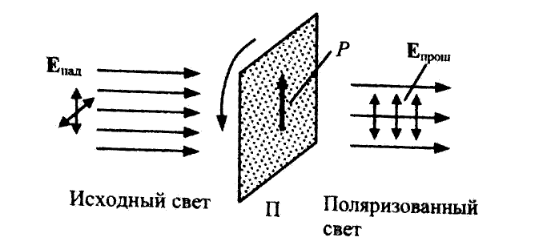
\includegraphics[scale=1]{polar.png}
    \label{fig:my_label}
\end{figure} 
Пусть на поляризатор падает частично поляризованный свет. Меняя ориентацию поляроида, находим, когда наблюдаются максимальная и минимальная интенсивности проходящего излучения.

Допустим, что свет содержит неполяризованную компоненту (естественный свет) и компоненту с линейной поляризацией. Если поляроид идеальный, то он "отсекает" половину интенсивности естественного света, поскольку все полярищации в нем представлены с равным весом. В то же время линейно поляризованная компонента либо полностью пропускается, либо полностью задерживается в зависимости от ориентации оси поляроида. Соответственно находим

\begin{equation*}
    I_{max} = \frac{1}{2}I_{\text{ест}} + I_{\text{пол}}, \hspace{10px} I_{min} = \frac{1}{2}I_{\text{ест}}.
\end{equation*}

В результате степень поляризации исследуемого излучения определяется по формуле

\begin{equation*}
    P = \frac{I_{\text{пол}}}{I_{\text{пол}} + I_{\text{ест}}} = \frac{I_{max} - I_{min}}{I_{max} + I_{min}}.
\end{equation*}

